\documentclass[two column]{article}
\usepackage[utf8]{inputenc}
\usepackage{graphicx}
\usepackage[dvipsnames]{xcolor}
\usepackage[colorlinks=true,linkcolor=Blue,hypertexnames=false]{hyperref}
\usepackage{braket}
\usepackage{bbold}
\usepackage{cite}
\usepackage{amssymb}
\usepackage{amsmath}
\usepackage{placeins}
\usepackage{subcaption}
\usepackage[qm]{qcircuit}
\usepackage[left=23mm,right=23mm,top=35mm,columnsep=15pt]{geometry}

\newcommand{\caro}[1]{\textcolor{red}{[#1]}}
\newcommand{\jovan}[1]{\textcolor{blue}{[#1]}}
\newcommand{\todo}[1]{\textcolor{orange}{[#1]}}
\newcommand{\steve}[1]{\textcolor{purple}{[#1]}}
\newcommand{\lang}[1]{\textcolor{brown}{#1}}
% green: just language, mostly too colloquial or grammar



\title{Nonabelian Braiding of Lattice Gauge Theory excitations on NISQ hardware}
\author{Jovan Jovanovic�, Carolin Wille, Daan Timmers and Steve H. Simon}
\date{February 2023}

\begin{document}

\maketitle
\begin{abstract}
Lorem Ipsum
\end{abstract}
\tableofcontents



\section{Proto-Introduction}

We have developed a framework of manipulating nonabelian excitations on top of a lattice gauge theory ground state realized on a digital quantum simulator.

The way braiding is implemented via local unitary gates is by keeping the copy of the non-local logical Hilbert space $\mathcal{H}_{\text{fusion}}$, alongside the Gauge Field degrees of freedom $\mathcal{H}_{\text{gauge}}$. The protocol is meant to couple the two systems such that once a specific measurement is preformed on the copy of the logical space and hence becoming disentangled from the gauge field, the gauge field is in the state that correspond to an appropriate space-time braiding of our anyons. The resulting state has: correct charge content, charges are in the correct fusion channel and the overall state is in the correct phase (in comparison to the vacuum).

Using this framework, we examine a couple of braiding experiments. The question we address is the plausibility of detecting the nonabelian braiding signatures given the levels of noise of current digital quantum simulators, Google's Sycamore chip in particular.

The reason for this choice is the suitable geometry of Sycamore for implementing surface codes and the availability of noise models. Also, this chip in particular has been instrumental in a number of recent experimental breakthroughs including, realization of toric code ground state \cite{}, nonabelina braiding of defected toric code anyons \cite{}; similar chips were also used to realize symmetry protected topological edge modes in Floquet driven circuits \cite{}.

In the next chapter, we will discuss the general framework of manipulating the nonabelian anyons of the quantum double model, with a brief overview of the model itself. Afterwards, we will propose a series of experiments one can compile for a digital quantum processor that showcase the nonabelian nature of these particles: non-unique fusion, nonabelian nature of the braid group represented by these particles and the non-trivial linking matrix. Following that, we will present the results of our noisy simulations, the goal of which are to show that these signatures are indeed measurable on the current quantum hardware. The last chapter will be dedicated to the discussion of future research in quantum simulation, having now ways to prepare arbitrary lattice gauge theory states.

\section{General Framework \caro{Quantum double models}}
\caro{\begin{itemize}
\item Add that QM double are a 
generalization of the toric code with vertex and plaquette terms
\item describe $A$ and $B$ in words
\item put a picture for each
\item general remark, no :, no arbitrary capitalisation and more careful with articles 
\end{itemize}}

Kitaev's quantum double models are a Hamiltonian formulation of lattice gauge theory, where the gauge group $G$ is finite, the gauge fixed by weakly \caro{what does weakly mean here?} requiring the Gauss' law be obeyed at every vertex and at a deconfinement fixed point (no electric field term).

The Hilbert space is defined for any fixed \textbf{directed} graph $\Lambda = \{V, E, P\}$ of vertices $V$, edges $E$ and plaquettes $P$. The basis vectors are labelled by all colourings of the edges by the elements of the group. \caro{would omit formula, strictly speaking would be $E\to G^{|E|}$., $\mathcal{H}_\text{gauge} = \text{Span}\{\ket{f}| f: E \rightarrow G\}$. }

The Hamiltonian is:
\begin{equation}
    H = -  \sum_{v \in V} B^{(e)}_v -  \sum_{p  \in  P}\sum_{g \in G} \frac{1}{|G|}A^{(g)}_p,
\end{equation}

The vertex terms are defined as follows:
\caro{how about just
$B_v(h) |g_1,g_2,g_3\rangle= \delta_{g_1 g_2 g_3,h} |g_1,g_2,g_3\rangle$ and a comment about starting point and orientation, likewise for $A_p(g) |g_1, g_2,\ldots \rangle = |g g_1, g_2 g^{-1}, \ldots \rangle$ plus a figure to illustrate orientation  }

\todo{Figure Ops: Showing the action of A and B operators.}

\begin{equation}
    B^{(h)}_v\ket{f} = \delta\left(\prod_{e \in \vec{E}_v}f(e)^{p_e} = h\right)\ket{f},\label{eqn:Bs_def}
\end{equation}


%with $\vec{E_v}$ being the set of legs incident on the vertex $v$ ordered such that the legs are going around the vertex clockwise, the product is taken within the group $G$, the ordering is important since the group may not be Abelian, $p_e = 1 \text{ or } -1$ depending on whether the leg is pointing into the vertex or out of the vertex. The delta function in the definition is the Kronecker delta.%

This term is diagonal in the basis described above. On the other hand, the plaquette term is
\begin{equation}
\begin{split}
    A^{(g)}_p\ket{f} = \ket{h},\\
   % h(e) = f(e) \text{, if } e \notin p \land e\notin \bar{p}, \\
    h(e) = g f(e) \text{, if } e \in p, \\
    h(e) = f(e) g^{-1} \text{, if } e \in \bar{p},
\end{split}\label{eqn:As_def}
\end{equation}
the plaquettes are oriented clockwise and if the orientation of the leg touching a plaquette is agreeing with the orientation of the plaquette we say $e \in p$, otherwise $e\in \bar{p}$.


\caro{move this paragraph to ground state section}
This term is not diagonal, but it does commute with the vertex term. In fact, all terms commute, hence we can diagonalize the Hamiltonian term-by-term and the leftover degeneracy depends only on the genus of the surface our graph is embedded in. \caro{They do matter somewhat if you use this for error correction. I would omit the following sentence.} Also, the relative strengths of the term do not matter and the dynamics that this Hamiltonian generates is trivial.

\caro{move the following paragraph in front of the Hamiltonian before the formulas}
As mentioned above, this is a gauge fixed lattice gauge theory in the Hamiltonian formalism. The vertex terms weakly enforce the Gauss' law, while the plaquette terms are the magnetic terms allowed by the gauge symmetry.


\caro{Move this paragraph to the anyon section or to measurement section}
The plaquette terms also generate the gauge transformations, i.e. if they act on a state that has a charge situated on a certain plaquette, they transform the state in accordance with the charge:
\begin{equation}
    A_p^{(g)}\ket{R, p; \mu} = \sum_\nu R(g)_{\mu}^{\nu}\ket{R, p;\nu},\label{eqn:tranfs}
\end{equation}
where $R$ is an irreducible representation of the gauge group $G$, while $\mu$ and $\nu$ are the vector indices.
We will use this fact in our protocol for charge measurement.

\subsection{The Ground State\caro{no need to give it its own subsection}}

The form of the ground state depends heavily on the geometry of the graph the theory is defined on.
As an example, depending only on the topology of the manifold in which we can embed our graph, the ground state can either be unique or degenerate.

For a case of the unique ground state on a graph embedded on $\mathcal{S}_2$ we have:
\caro{This is not right, you need to make sure that the GL respecting terms all come with the appropriate weights in the superposition. Probably easiest construction is to use empty lattice and apply all plaquette terms.}
\begin{equation}
    \ket{G.S.} \propto \sum_{f \in \text{G.L.}} \ket{f},
\end{equation}
where G.L. is a set of all labellings which obey the Gauss law, i.e. are not annihilated by any $B_v^{(e)}$.\caro{omit the formula}
\begin{equation}
    \text{G.L.} = \{f: E \rightarrow G |\prod_{e \in \vec{E}_v}f(e)^{p_e} = e \text{ for all } v \in V\}.
\end{equation}

\caro{Move the discussion about GS preparation to Introduction and to the geometry section, here is not the right place}
There was a lot of work done on the question of preparing topologically ordered states on quantum simulators \cite{}. We, however, will not be using any clever method but will restrict ourselves to very simple (and small) geometries where the preparation is trivial. This is due to various qubit number and circuit depth restrictions imposed on us by the state of NISQ devices, which will become clear in the following two sections, hence we will not elaborate further for now. 

\subsection{Excitations}
\caro{Move this to GS section}
As we saw, the Hamiltonian is made out of commuting terms, moreover, it is easy to see that they are projectors. The ground state is stabilized by all projectors:
\begin{equation}
\begin{split}
    A^{(g)}_p \ket{\psi} = \ket{\psi},\\
    B^{(e)}_v \ket{\psi} = \ket{\psi},
\end{split}\label{eqn:ground_state}
\end{equation}
true for all $v \in V$ and $p \in P$.

\caro{'one can imagine' is not very scientific language. replace by sth like 'the excited states are given by..'}


Therefore, one can imagine that the elementary excitation above the ground state will disturb one or more of the equations above.

To get a better handle on this question, one needs to look at the algebra spanned by these vertex and plaquette operators. But first, we need to put vertices and plaquettes on an equal footing. This is done by pairing plaquettes and adjacent vertices one-to-one into sites, of course either some vertices or some plaquettes will be left over depending on the exact geometry of the lattice. 

Let's label the sites by $s_i = (v_i, p_i)$ such that: $A_{s_i}^{(g)} = A_{p_i}^{(g)}$ and $B_{s_i}^{(h)} = B_{v_i}^{(h)}$. 

Operators on different sites commute trivially, while on each site we have the following:
\begin{equation}
    \begin{split}
        A_s^{(g)}A_s^{(h)} = A_s^{(gh)}, \\
        B_s^{(g)}B_s^{(h)} = \delta_{g,h} B_s^{(h)},\\
        A_s^{(g)}B_s^{(h)} = B_s^{(ghg^{-1})}A_s^{(g)}.
    \end{split}
\end{equation}

This is the on-site representation of a certain algebra known as the quantum double of a finite group $G$, $D(G)$. This algebra does not depend on the exact grouping of plaquettes and vertices into sites.

The on-site excitations are labelled by the irreducible representations of this algebra \cite{}, and the ground state can be viewed as one with a trivial (charge free) representation at each site, therefore by the definition of the trivial representation satisfying Eq.~\eqref{eqn:ground_state}.

\caro{At some point we need to introduce the notion of pure charge, pure flux and a dyon, we should state the simplified expressions for pure charge and pure flux, and the notion of generalized conjugation in the dyon case, as we use this later on.}

To illustrate this point, we will now describe the irreducible representation of this algebra. The representations are labelled by two objects, the conjugacy class $C$ of the group $G$ and an irreducible representation $\chi$ of the centralizer of the class representative $Z(r)$, with $r \in C$. The irreducible representation, is then labelled by $(C, \chi)$, the vector space on which $(C, \chi)$ acts is spanned by a basis $\ket{\mu} = \ket{c, i}$, where $c \in C$ and $i \in \{1, 2, \ldots, \text{dim}\chi\}$.

The action of the algebra generators on this vector space is then:
\caro{what happens with $i,i'$ in the first line?}
\begin{equation}
    \begin{split}
        B^{(h)}_{\mu\nu}=\bra{c, i} B^{(h)} \ket{c', i'} = \delta_{c, h} \delta_{c, c'}, \\
        A^{(g)}_{\mu\nu} = \bra{c, i} A^{(g)} \ket{c', i'} = \delta_{c,gc'g^{-1}} \Gamma^\chi_{ii'}(q_{c}^{-1}gq_{c'}),
    \end{split}
\end{equation}
where $\Gamma$ is the $\chi$-representation matrix, $q_c$ are the coset representatives of $G/Z(r)$. They make sure that $q_c^{-1}gq_{c'} \in Z(r)$ for all $g$ such that $c = gc'g^{-1}$.
\caro{omit:
These representation matrices are going to play a central role in our protocols for creating and manipulating anyons.}

As an example, the aforementioned vacuum (or trivial) representation, labelled by $(\{e\}, \mathbb{1})$, is one-dimensional and spanned by $\ket{e, 0}$:
\begin{equation}
    \begin{split}
        B^{(h)}\ket{e, 0} = \delta_{h,e}\ket{e, 0},\\
        A^{(g)}\ket{e, 0} = \ket{e,0},
    \end{split}
\end{equation}
hence by Eq.~\eqref{eqn:ground_state} we see that the ground state is such that every site houses a trivial representation (hence the name, vacuum).

\subsection{Ribbon Operators}

The excitations mentioned in the previous chapter are created in pairs from the vacuum. To see why, imagine we take the ground state and change the \caro{first time you use the word flavour, needs to be defines} flavour of one of the legs $f(e_0) \rightarrow gf(e_0)$, this action disturbs two vertex operators $B^{(e)}_{e_0^+}$ and $B^{(e)}_{e_0^-}$ on each end of the leg $e_0$.

There exists a set of such line/ribbon operators that when acted upon a ground state create two excitations on both of its ends. These operators are labelled by the elementary excitations. 

If the ribbons are closed, they leave the ground state unchanged, since there are no ends. Moreover, they span all (loop) operators that leave the ground state invariant, it is in that way that the quantum double ground state knows about the quasiparticle spectrum.

The ribbon operators are constructed in Ref \cite{}. These operators represent a planar diagram algebra generated by the specific Braiding Tensor Category (BTC) and hence were conceived as a model that can perform fault-tolerant quantum computing by the means of braiding anyons. 

However, even though the braid group itself is universal \cite{} its image on this planar diagram algebra is finite, hence non-universal. For some gauge groups it can be made universal by the addition of measurements, but it will not be the case for our example.

\caro{remove unnecessary words] Another issue is the fact that }the ribbon operators are not unitary. If the anyons have an internal dimension larger than one, the operators that create and manipulate the excitations are non-local projectors (or unitarily related to projectors). \caro{informal language In Ref. \cite{} the group got around this issue }by the means of unitary lattice deformations, rotating from a state with a set of nonabelian anyons on one graph to another state with the same anyon content but defined on another graph, hence they were able to move the internal dimension-1/2 (majorana fermions) anyons unitarily. However, these are extrinsic and static lattice defects on top of a theory that is an Abelian $\mathbb Z_2$ gauge theory, hence, the nature of theirs and our nonabelian anyons is different.

\subsubsection{Application Scheme}
We are going to describe a scheme by which we implement these non-local projecting ribbon operators.

It starts by identifying the anyon type and the representation associated with them. 

Say we have a ribbon of type $(C, \chi)$ of dimension $d = \text{dim}(C, \chi)$. There are a couple of interpretations of the dimension $d$, one is that the anyons carry an internal spin-like degree of freedom encoded in the gauge field itself, another one is that the fusion outcomes span a $d\times d$ space of the representation $(C, \chi) \otimes (C, \chi)$, individual outcomes being the subspaces in the Clebsch-Gordan decomposition.

Note that the fusion outcome is a non-local degree of freedom once the anyons are separated, this being the main idea of fault-tolerant topological quantum computing.

We, however, require storing this information locally since we need to do measurements on this space as we move the anyons. This is done by keeping one auxilliary qudit per anyon/end of the ribbon.

\caro{remove:The last point before we describe the algorithm is that } every ribbon is made up from two kinds of elementary triangles \caro{add a comment that the details of the operators depend on orientations etc as explained in Fig. sth, and omit the rest of this paragraph}, one set that follows a leg and another that cuts a leg. There are also two kinds of orientations, since the ribbons are directed. Moreover, the leg in the triangle can be oriented in two ways. Finally, there are two ways to glue a triangle to a ribbon, continuing it forwards or backwards. See Figure \ref{} for the breakdown of 16 types of elementary triangles making up a ribbon.

\todo{Figure Ribbon Example: An example of a ribbon decomposed into elementary triangles}

\todo{Figure Triangles: Figure showing the 16 types of triangles: [(I, II), (R, L), (in, out), (f, b)]}

\caro{You do that sequentially, i.e., not just 'for all $t_i$' but one after another. Also, would be easier to just talk about a forward moving ribbon where you only have $|c,i\rangle$ and $|g\rangle$ and then consider backwards in an appendix}
\textbf{The algorithm} that creates two anyons along a ribbon path $R$ made up from a set of triangles $R = \{t_1, t_2, \ldots, t_N\}$ in the internal state: $\ket{\alpha; \beta} = \ket{c', i'; c, i}$ i.e. applying $F_{\alpha, \beta}^{(C,\chi)}(R)$ is:

\textbf{1.} Initialize the two \caro{auxiliary} qudits in the states $\ket{\alpha, \beta}$ 

\textbf{2.} For each $t_i$ in R do one of the following unitaries depending on the type of the triangle:
\caro{drop the [II,R, in f] here}

[I, R, in, f]: $\ket{c', i';c, i}\ket{g}_{t_i} \rightarrow \ket{c', i';c, i}\ket{cg}_{t_i}$

[II, R, in, f]: $\ket{\alpha;\beta}\ket{g}_{t_i} \rightarrow \sum_\gamma A_{\gamma\beta}^{(g)}\ket{\alpha;\gamma}\ket{g}_{t_i}$

$\ldots$ \footnote{For the rest of the rules consult the Appendix \ref{}, $\ket{g}_{t_i}$ is the state of the physical leg that belongs to the elementary triangle $t_i$.}

\textbf{3.} Project the ancillary qudits to a Bell-pair state \caro{save that comment for later (measure and post-selection, or error correction where possible):} $\bra{\Phi^+} = \frac{1}{\sqrt{d}}\sum_\nu \bra{\nu; \nu}$

This creates a pair of excitations on the ends of a ribbon $R$ of type $(C, \chi)$ in an internal (fusion) state $\ket{\alpha, \beta}$. This way, we have started building up the ribbon n from start-to-finish using only forward-type elementary triangles. Similarly, we could have started in the middle and extend parallely both forward and backwards with appropriate types of elementary triangles\caro{omit formulas}:

\textbf{2.} Alternative:

[I, R, in, b]: $\ket{c', i';c, i}\ket{g}_{t_i} \rightarrow \ket{c', i';c, i}\ket{c'g}_{t_i}$

[II, R, in, b]: $\ket{\alpha;\beta}\ket{g}_{t_i} \rightarrow \sum_\gamma A_{\alpha\gamma}^{(g)}\ket{\gamma;\beta}\ket{g}_{t_i}$

$\ldots$

As we can see the operation is sequential so at best the depth of a circuit implementing this is $\mathcal{O}(|R|)$, with the best depth achieved by starting at the middle and growing it both ways.

Of course, we can make this constant depth by separating the main Ribbon into $|R|$ smaller ribbons which however requires $|R|$ pairs of qudits and Bell-pair measurements \caro{remove, colloquial:, a nightmare for post-selection/error correction (which for the case of $D_4$ theory can be done).}

To interpret what we have here, let us look at the quantum recourses. We have the qudits representing the matter $\mathcal{H}_{\text{matter}}$ and the ancillary bits representing the internal state of the anyons, or the fusion space, $\mathcal{H}_{\text{ancilas}} \equiv \mathcal{H}_{\text{fusion}}$ which is already embedded non-locally in  $\mathcal{H}_{\text{matter}}$.

\caro{remove So, }the two types of triangles couple the two spaces in two different ways, for type \caro{ just say type I. and type II [I, , , ]} the $\mathcal{H}_{\text{ancilas}}$ controls an action on $\mathcal{H}_{\text{matter}}$ and for type [II, , , ] it is the other way around. After the measurement that disentangles the redundant copy of $\mathcal{H}_{\text{fusion}}$ the $\mathcal{H}_{\text{matter}}$ is left in a state with the ribbon operator imprinted on it \caro{e.g. 'as signalled by the'}, topological charge, braiding amplitude and phase.

\subsection{Charge Measurement}
\caro{Explain the idea of reduced charge measurement in words, i.e., get partial information and combine the partial information for different $H$ to deduce charge}

The last important element of our toolkit for probing topological order is the measurement protocol for topological charge of the gauge field configuration.

The ideal charge measurement would differentiate any type of excitation on any site, such measurement is associated with the following set of projectors \cite{}:
\begin{equation}
    P_s^{(C, \chi)} = \frac{\chi(e)}{|Z(r)|}\sum_{c \in C}\sum_{z \in Z(r)}\chi^*(z)B_s^{(c)}A_s^{(q_c z \bar{q}_c)},
\end{equation}
for each representation of the $D(G)$.

This, however, operators $A^{(g)}_s$ require a group multiplication applied to all legs in $s$'s plaquette. As we will show in the \caro{replace by 'case of non-abelian groups'} specific case of $G = D_4$ is prohibitively expensive.

\subsubsection{Reduced Charge Measurement}
\caro{general comment: just talk about the reduced charge measurement, make the purpose of it clear in the first few sentences: reduced circuit depth is traded for only gaining partial information because measurement outcomes for a single subgroup are compatible with several charges, repeating the measurement for different subgroups allows to deduce charge uniquely for examples considered (D4, Q8), skip all of the following until}
We will present a simplified scheme that circumvents the large circuit depths of implementing a general charge measurement.
We begin by noting that the flux can be just readout from complete projective measurement of the physical degrees of freedom:
\begin{equation}
    O = \sum_{f \in F.} \ket{f}\bra{f},
\end{equation}
with $F. = \{f: E \rightarrow G\}$. 
Once we get a certain labelling as an outcome, $\ket{f}$ we can just classically compute the flux.
\caro{next sentence unclear}
This, however, destroys the charge information, so we need to preserve it in a set of ancillary bits we read out in addition to all the physical legs.

Also, we would like to do this cheaply.

\caro{here}
\caro{Insert paragraph from above and clarify what $\mu$ is}
We start with a state that has pure charge on a plaquette $p$, $\ket{R, p; \mu}$.
Given a subset of the group $H \subset G$, we \caro{this is a protocool. 'can implement' $\to$'perform'} can implement a group multiplication around the plaquette $p$ but only for the group elements in $H$.
This restriction is the key to greatly reduce the complexity of the circuit depth\caro{the figure here is too early and does make little sense, we need to introduce the encoding first, we also need to explain why toffoli are so costly, bc here it looks like depth 6 to depth 3}, see Figure \ref{fig:restMult} for an example.

\begin{figure}
\begin{equation*}
\Qcircuit @C=0.5em @R=0.7em @!R{
\lstick{m} & \qw & \ctrl{3} & \qw & \qw & \qw & \qw\\
\lstick{R} & \ctrl{2} & \qw & \ctrl{3} & \ctrl{3} & \qw & \qw\\
\lstick{R^{2}} & \qw  & \qw & \qw & \qw & \ctrl{3} & \qw
\\
\lstick{\quad m} &  \ctrl{2} & \targ & \qw & \qw & \qw & \qw\\
\lstick{R} & \qw & \qw & \ctrl{1} & \targ & \qw & \qw\\
\lstick{R^{2}} & \targ & \qw & \targ & \qw & \targ & \qw
}\qquad\qquad
\Qcircuit @C=0.5em @R=0.7em @!R{
\lstick{mR} & \ctrl{2} & \ctrl{3} & \qw & \qw\\
\lstick{R^{2}} & \qw  & \qw & \ctrl{3} & \qw
\\
\lstick{\quad m} &  \targ & \qw & \qw & \qw \\
\lstick{R} & \qw & \targ & \qw & \qw\\
\lstick{R^{2}} & \qw & \qw & \targ & \qw
}\qquad\qquad
\Qcircuit @C=0.5em @R=0.7em @!R{
\lstick{R^{2}} & \qw  & \ctrl{3} & \qw
\\
\lstick{\quad m} &  \gate{X} & \qw & \qw \\
\lstick{R} & \qw & \qw & \qw\\
\lstick{R^{2}} & \qw & \targ & \qw
}
\end{equation*}

    \caption{Group multiplication circuits: $U_{\text{CM}}:\ket{g,h} \rightarrow \ket{g,gh}$. Left: Both $g$ and $h$ are unrestricted to be any element of the group $G$, the first three qubits encode the first elements and the second three the second element. Center: The first element is restricted to be in $H_{mr}$ subgroup and is encoded by just the first two qubits. Left: The first element is restricted to be in $C_m$ conjugacy class and is encode by just the first qubit. Note the significant simplification in the circuit complexity when the inputs are restricted.}
    \label{fig:restMult}
\end{figure}

With \caro{no 'the', just write Eq. (4)}the equation \ref{eqn:tranfs} in mind, we propose the following protocol:

\textbf{The algorithm} for the reduced pure charge measurement on a plaquette $p$ given a state $\ket{R, p; \mu}$:

\textbf{1.} Prepare ancillary qudits to encode the elements of $H$, the joint state is then $\sum_{h\in H}\ket{h}_{a}\ket{R, p; \mu}$

\textbf{2.} Controlled on the state of the ancillary qudit $a$ we multiply the elements $h$ into legs touching the plaquette $p$, i.e. apply the plaquette operator $A_p^{(h)}$:

\begin{equation}
\begin{split}
    \sum_{h\in H}\ket{h}_{a}\ket{R, p; \mu} \rightarrow \sum_{h\in H}\ket{h}_{a}A_p^{(h)}\ket{R, p; \mu} = \\ \sum_{h\in H}\sum_\nu \ket{h}_{a}R(h)_\mu^\nu\ket{R, p; \nu}
\end{split}
\end{equation}

\textbf{3.} We perform the appropriate unitary on the ancillary bit to decouple it from the matter, with this act imprinting the information about the charge on the ancillary qudit.

As an illustration, let's take $H = G$ and the unitary be a following transformation:
\caro{is it possible to declutter this a bit?}
\begin{equation}
U_a = \sum_{h'\in G} \sum_{R'; \alpha, \beta} R'(h')_\alpha^\beta  \ket{R'; \alpha, \beta}_a\bra{h'}_a,
\end{equation}
with the second sum running over irreducible representations of $G$, $R'(h')_\alpha^\beta$, and over the matrix indices.
The unitarity of this matrix is guaranteed by the Schur's orthogonality theorem, it is the said theorem that also guarantees that this unitary will decouple matter and ancillary degrees of freedom:

\begin{equation}
    \begin{split}
        \sum_{h\in G}\sum_\nu \ket{h}_{a}R(h)_\mu^\nu\ket{R, p; \nu} \rightarrow \\
        \sum_{h\in G}\sum_\nu\sum_{R'; \alpha, \beta} \ket{R'; \alpha, \beta}_{a}R'(h)_\alpha^\beta R(h)_\mu^\nu\ket{R, p; \nu} = \\
        \sum_\nu \ket{R; \mu, \nu}_{a}\ket{R, p; \nu},
    \end{split}
\end{equation}
the last equality following from the sum over the group elements $h$ and Schur's orthogonality theorem, $\sum_{g}R'(g)_\alpha^\beta R(g)_\gamma^\delta = |G|\delta_{RR'}\delta_{\alpha\gamma}\delta_{\beta\delta}$.

\textbf{4.} Measure the ancillary qudit.

In the case above, the result of the measurement is a label $(R, \mu, \nu)$, representing the charge, the internal state before the measurement and the internal state after the measurement.

This is an example of full charge measurement, giving the full charge information. However, it is possible to get partial charge information if instead of a full group we use a subgroup $H \subset G$ and one of its irreducible representations to construct the decoupling unitary $U_a$ as:
\begin{equation}
    U_a = \sum_{h \in H} \sum_{R_H} R_H(h)_\alpha^\beta\ket{R_H; \alpha, \beta}_a\bra{h}_a,
\end{equation}
where the sum goes over $R_H$ the irreps of $H\subset G$.

By partial charge information, we mean that the result of the measurement protocol is not a single charge, but a set of possible charges that may be there at a site we are probing.

We may then repeat the procedure using different subgroups of $G$ to gather further information on the charge in the hope that we may be able to deduce the full charge information for this series of partial charge information.

This relies on partial orthogonality of character tables of a group and its subgroup, and is best explored in the specific cases below. 

\subsubsection{Specific example of $D_4$}

In this section, we explore the reduced charge measurement in the case of $D_4$ gauge group.
Limiting ourselves to only pure charges, remembering that the flux component can be directly read out, we have five possibilities for topological charge on a site: $0$, $\Sigma_r$, $\Sigma_m$, $\Sigma_{mr}$ and $\Sigma_{\epsilon}$. Please consult the Appendix \ref{} for the list of all representations of $D(D_4)$.

The traces of the representation matrices $R(g)_\alpha^\beta$ for the five flavours are given in Table \ref{tab:char}. This is just a character table of $D_4$ and the association between the irreps and topological charges mentioned above are: $1 \rightarrow 0$, $\alpha_x \rightarrow \Sigma_x$ and $\epsilon \rightarrow \Sigma_\epsilon$.

\begin{table}[h]
\centering    \begin{tabular}{c|c c c c c }
         %\hline
         $D_4$ & $\mathcal C_e$ & $\mathcal C_{r^2}$ & $\mathcal C_{r}$ & $\mathcal C_m$ & $\mathcal C_{mr}$ \\
         \hline
         $1$ & 1 & 1 & 1 & 1 & 1 \\
        % \hline
         $\alpha_r $& 1 & 1 & 1 & -1 & -1  \\
         %\hline
         $\alpha_{m}$ & 1 & 1 & -1 & 1 & -1  \\
         %\hline
         $\alpha_{mr}$ & 1 & 1 & -1 & -1 & 1  \\
         %\hline
         $\epsilon$ & 2 & -2 & 0 & 0 & 0  \\
         %\hline 
    \end{tabular}
    \caption{Character table of $D_4$.}\label{tab:char}
\end{table}

All the proper subgroups of $D_4$ are abelian, hence all the $R_H$ are one dimensional, this means that the measurement outcome of the reduced charge measurement is just the irrep label $(R_H)$.

We will focus on the three four element subgroups $H_r = \{e, r, r^2, r^3\} \equiv \mathbb{Z}_4$, $H_r = \{e, r^2, mr^2, mr^2\} \equiv \mathbb{Z}_2 \times \mathbb{Z}_2$ and $H_r = \{e, r^2, mr, mr^3\} \equiv \mathbb{Z}_2 \times \mathbb{Z}_2$.

The partial orthogonality of irreps of $D_4$ and these three groups is captured in the quantity: $ \braket{R, R_H} = \sum_h \chi_R(h)\chi_{R_H}(h)$. This is shown in Table \ref{tab:red_ch}, see the Appendix \ref{} for the list of irreps of subgroups of $D_4$.


\begin{table}[h]
\centering
\begin{tabular}{l|lllll}
  $\braket{R_{H_m}, R}$ & $1$ & $\alpha_{r}$ & $\alpha_{m}$ & $\alpha_{mr}$ & $\alpha_{\epsilon}$ \\ \hline
$(1,1)$ & 4   & 0            & 4             & 0               & 0                   \\ 
$ (1,-1)$ & 0   & 4            & 0             & 4               & 0                   \\ 
$(-1,1)$ & 0   & 0            & 0             & 0               & 4                   \\ 
$(-1,-1)$ & 0   & 0            & 0             & 0               & 4                   \\ 
\end{tabular}
\begin{tabular}{l|lllll}
  $\braket{R_{H_{mr}}, R}$ & $1$ & $\alpha_{r}$ & $\alpha_{m}$ & $\alpha_{mr}$ & $\alpha_{\epsilon}$ \\ \hline
$(1,1)$ & 4   & 0            & 0             & 4               & 0                   \\ 
$ (1,-1)$ & 0   & 4            & 4             & 0               & 0                   \\ 
$(-1,1)$ & 0   & 0            & 0             & 0               & 4                   \\ 
$(-1,-1)$ & 0   & 0            & 0             & 0               & 4                   \\ 
\end{tabular}
\begin{tabular}{l|lllll}
  $\braket{R_{H_r}, R}$ & $1$ & $\alpha_{r}$ & $\alpha_{m}$ & $\alpha_{mr}$ & $\alpha_{\epsilon}$ \\ \hline
$1$ & 4   & 4            & 0             & 0               & 0                   \\ 
$-1$ & 0   & 0            & 4             & 4               & 0                   \\ 
$i$ & 0   & 0            & 0             & 0               & 4                   \\ 
$-i$ & 0   & 0            & 0             & 0               & 4                   \\ 
\end{tabular}
\caption{Partial orthogonality of $D_4$ with respect to its three four-element subgroups.}
\label{tab:red_ch}
\end{table}

The Table \ref{tab:red_ch} is to be interpreted as follows, the outcome of a reduced charge measurement is a label $R_H \in \{(1,1), (-1,1), (1,-1), (-1,-1)\}$, in the case of $H = H_m$ for example. \caro{What about the $\pm i$ outcomes for $H_r$? we can't measure $\pm i$.} The outcomes, hence, are represented by rows in this table and all non-zero elements correspond to a possible topological charge given that measurement outcome. Hence, we can see that each charge has a unique set of outcomes of the reduced charge measurement for these three subgroups.
\caro{We are more interested in the inverse direction, namely, the result $\{(1,-1); (1,-1); 1\}$ is only compatible with charge $\Sigma_r$.}
As an example, let's take $\Sigma_r$, upon the three measurements this charge can only produce the following set of results $\{(1,-1); (1,-1); 1\}$ for subgroups $H_m$, $H_{mr}$, $H_r$ respectively. \lang{Same, holds for others.}

The main advantage of doing these three measurements instead of a full charge measurement is two fold, both the controlled multiply unitary $U_{\text{CM}}: \ket{h, g} \rightarrow \ket{h, hg}$ and the decoupling unitary $U_a$ are much simpler if we restrict ourselves to $h \in H \subset G$.


\section{Braiding Experiments and Numerical Results}

In this chapter, we will present a set of braiding protocols that fully demonstrate the braiding statistics of the $D_4$ lattice gauge theory excitations. These also generate all the braiding amplitudes of the braiding protocols, however direct evaluation of longer protocols on current NISQ hardware is prohibited by the limitation on the circuit depth imposed by the noise, as the reader will see in the next chapter. 

The main experiments showcasing the nonabelian nature of the excitations are as follows:

i) anyon fusion; \lang{the fusion outcome doesn't have} unique topological charge,

ii) nonabelian braiding; the braiding amplitude changes as we change the order of braids,

iii) \caro{full S- and T-matrix measurement; this generates the complete UTC data that specifies any braiding amplitude.
%Technically speaking, the UMTC data is not captured by S and T matrix alone
}
 
It is easy to obtain the results of the first two experiments from the result of the last one, however it is useful to consider the two foundational phenomenological facts pertaining to the nonabelian anyons in separate points.

\subsection{$D_4$ Specifics: Encoding, Ribbon operators and Charge Measurements}

In this section, we will discuss the group element encoding and group operation circuits \lang{based around} this encoding.
The states of the gauge field are characterized by group element labelings of the legs of the graph.
In general, our degrees of freedom are group valued.
The cardinality of $D_4$ is 8, hence we need three qubits to encode a group element.
We chose the following map
\begin{equation}
    \ket{g} \equiv \ket{a}_m\ket{b}_r\ket{c}_{r^2} \iff g = m^a r^b (r^2)^c,
\end{equation}
where $a,b,c \in \{0,1\}$ and $r$ is the $90^{\text{o}}$ rotations and $m$ is the reflection.

When encoding the internal space of the anyon, which we need for our ribbon operator protocol, we note that the basis also include a group element component: $\ket{\nu} = \ket{c, i}$, where $c \in C_x$, for some conjugacy class.
The elements of a conjugacy class are also encoded similarly, for example, $C_r = \{r, r^3\}$:
\begin{equation}
    \ket{c} \equiv \ket{a}_{r^2} \iff c = m^0r^1(r^2)^a,
\end{equation}
using only one qubit.

This also hold for encoding elements of a subgroup:
\begin{equation}
    \ket{h} \equiv \ket{a}_r\ket{b}_{r^2} \iff h = m^0r^a(r^2)^b,
\end{equation}
for the example of $h \in H_r$.

These \caro{restrictions%these are not really restrictions, maybe say that we often just need to multiply with elements from a certain conjugacy class as indicated by the ribbon operator prescriptions in Eq. sth and that for this purpose we can use a single qubit and a circuit that is much shorter than the general group multiplication circuit.
} 
not only reduce the number of bits needed, but also greatly reduce the complexity of circuits implementing various group operations.

Lastly, there is no natural way to encode the representations of the subgroups $R_H$, hence for $H_m$ and $H_{mr}$ we will use:
\begin{equation}
    \ket{(-1)^a,(-1)^b} \equiv \ket{a,b}.
\end{equation}


\caro{
Let us return to circuits implementing group operation. We already presented some in Figure \ref{fig:restMult} in order to showcase the great simplifications of group multiplication when someone restricts the domain of the multiplication unitary, $U_{\text{CM}}: \ket{g, h} \rightarrow \ket{g, gh}$, from the full group to a subgroup and a single conjugacy class.
%This is the first time we actually discuss circuits. How about we start off with 'we need group multiplication and conjugation', these are the general circuits that do these two operations, they are long bc they involve x number of tofollis. however for ribbons we need only group multiplication for elements of conjugacy class which reduces circuit depths significantly, then include fig:restMult
}

This is one of the main facts that allows us to greatly simplify many circuits related to ribbon operators and reduced charge measurement. However, the direct ground state preparation \lang{doesn't} benefit from these simplifications.

The \lang{rest of multiplication unitaries are compiled} in the Appendix \ref{}.

We saw that the ribbon operators are made up from two types of elementary triangles. The first require group multiplication maps, restricted to a single conjugacy class, from the auxiliary degree of freedom onto the matter. The other are acting the other way around, implementing a specific representation of the group transformation onto the auxiliary degree of freedom controlled by the matter.

\caro{To illustrate this %rewrite, let us say exactly what we illustrate, we present an example of the circuits needed to apply a dyon-ribbon and a pure flux ribbon
}, let us examine two different ribbon flavours, for the rest consult the Appendix \ref{}. 
The two flavour are on the opposite ends of the complexity scale. 
The first will be the pure flux $\Psi_m \equiv (C_m, (1,1))$ and the second will be the dyon $\tilde{\Phi}_m \equiv (C_m, (-1, -1))$.
The representation matrices $A^{(g)}$ for the two representations are shown in Table \ref{tab:somereps}.


\begin{table}[]
    \centering
    \begin{tabular}{|l||l|l|l|l|l|l|l|l|}
    \hline
  $A^{(g)}$ & $e$ &   $r$ & $r^2$ & $r^3$ &  $m$ & $mr$ & $mr^2$ & $mr^3$ \\
\hline\hline
 $\Psi_{m}$ &$\mathbb{1}$&  $\sigma_x$ & $\mathbb{1}$&  $\sigma_x$ & $\mathbb{1}$& $\sigma_x$ &  $\mathbb{1}$&   $\sigma_x$ \\\hline
 $\tilde{\Phi}_{m}$ &$\mathbb{1}$&$i\sigma_y$ &$-\mathbb{1}$& $-i\sigma_y$ &$-\sigma_z$ &$-\sigma_x$ &  $\sigma_z$ &   $\sigma_x$ \\\hline
\end{tabular}
    \caption{$A^{(g)}$ matrices for $\Psi_m$ and $\tilde{\Phi}_m$ representation of $D(D_4)$.}
    \label{tab:somereps}
\end{table}

These two representations are two-dimensional, anyons are nonabelian and have an internal state space spanned by vectors: $\{\ket{m; ++}, \ket{mr^2; ++}\}$ for $\Psi_m$ and $\{\ket{m; --}, \ket{mr^2; --}\}$ for $\tilde{\Phi}_m$.
This space is encodable with a single auxiliary bit for each anyon, $\ket{a}_{\text{aux}} \equiv \ket{m(r^2)^a; \sigma\sigma}$.

The matter will act on this space every time an anyon crosses some leg $i$ via $U: \ket{a}\ket{g}_i \rightarrow (A^{(g)}\ket{a})\ket{g}_i$, which we need to compile.
The circuits for this operation are shown in Figure \ref{fig:genConj}.
It is easy to check that these circuits agree with the representation matrices given in Table \ref{tab:somereps}.

\begin{figure}
\begin{equation*}
\begin{split}
\Qcircuit @C=0.5em @R=0.7em @!R{
\lstick{m} & \qw & \qw \\
\lstick{R} & \ctrl{2}  & \qw \\
\lstick{R^{2}} & \qw  & \qw \\
\lstick{\text{aux}} &  \targ & \qw
}\qquad\qquad
\Qcircuit @C=0.5em @R=0.7em @!R{
\lstick{m} & \ctrl{3} & \qw & \qw & \qw\\
\lstick{R} & \qw & \ctrl{2} & \qw & \qw\\
\lstick{R^{2}} & \qw  & \qw & \gate{Z} & \qw\\
\lstick{\text{aux}} & \gate{-Z}  & \gate{jY} & \qw & \qw 
}\qquad\qquad
\Qcircuit @C=0.5em @R=0.7em @!R{
\lstick{m} & \gate{X} & \qw \\
\lstick{R} & \qw  & \qw \\
\lstick{R^{2}} & \targ  & \qw \\
\lstick{\text{aux}} &  \ctrl{-1} & \qw
}
\end{split}
\end{equation*}

    \caption{\caro{need to explain jY} Circuits \lang{involved in anyon manipulation, ribbon operators}. The first three qubits encode the physical, group valued, degree of freedom of the gauge field; the last qubit encodes the auxiliary bit representing the internal state of the (two-dimensional) anyon. Left: the conjugation unitary $U: \ket{c}\ket{g}_i \rightarrow \ket{gcg^{-1}}\ket{g}_i$ used when the pure flux $\Psi_m$ crosses a leg $i$. Middle: the generalized conjugation unitary $U: \ket{c}\ket{g}_i \rightarrow (A^{(g)}\ket{c})\ket{g}_i$ used when a dyon $\tilde{\Phi}_m$ crosses a leg $i$. Right: multiplication unitary $U: \ket{c}\ket{g}_i \rightarrow\ket{c}\ket{cg}$ used when either of the two anyons moves along a physical leg $i$. Note: $\ket{c} = \ket{a}_{\text{aux}} \iff c = m(r^2)^a$, for $a\in\{0,1\}$.}
    \label{fig:genConj}
\end{figure}

These elementary operations, with a couple of additional edge cases (see Appendix \ref{}), allow us to apply ribbon operators along any path.
We can create, move/braid and annihilate anyons by means of \lang{these couple simple circuits.}
\caro{However, as mentioned there are schemes that have better scaling for solvable gauge groups (such as $D_4$)\cite{}, but, the overhead makes them less preferable for such small systems and the universality of this approach makes it a good avenue for further exploration.
% schemes for what exactly?
}
Lastly, we 


\subsection{Geometry and Ground State Preparation}
A suitable choice of geometry can eliminate two of the main challenges of implementing the braiding protocols on a NISQ device.

\caro{
%We do not want to add having no long range entanglement as an advantage, rephrase this. Also, not everyone might now immediately that long range entanglement is 1:1 with long circuits (even though it is kind of the definition)
First, the circuit depth, a suitable choice of geometry can make the ground state not long range entangled, hence easy to prepare unitarily. However, one must not make the graph too simple for braiding.}

Second, the size of NISQ chips, one cannot embed a big two-dimensional graph on circa 50 qubits while leaving room for ancillary bits for ribbon operators and charge measurement.

We will hence, for the majority of our result, focus on what we call a braiding ladder. 
This geometry is shown in Figure \ref{fig:latticeGS}.

\begin{figure*}
    \begin{subfigure}{0.7\textwidth}\hfill
    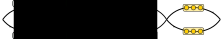
\includegraphics[width=\linewidth]{Figures/glasses.pdf}
    \vspace{0.05cm}
  %  \caption{Lattice}
    %\label{fig:gen_geom}
    \end{subfigure} %
    \hfill
    \begin{subfigure}{0.25\textwidth}
    \begin{equation*}
    \Qcircuit @C=0.2em @R=0.2em {
\lstick{m} & \gate{H} &       \ctrl{3} & \qw & \qw &\qw \\
\lstick{R} & \gate{H} &   \qw & \ctrl{3} & \qw & \qw \\
\lstick{R^{2}} & \gate{H} &  \qw & \qw & \ctrl{3} & \qw 
% \inputgrouph{1}{3}{2.2em}{\ket{h}}{2.5em}
\\
\lstick{\quad m} &  \qw &   \targ & \qw & \qw & \qw \\
\lstick{R} & \qw&   \qw &  \targ & \qw & \qw \\
\lstick{R^{2}} & \qw & \qw&   \qw &  \targ & \qw 
% \inputgrouph{4}{6}{2.2em}{\ket{g}}{2.5em}
}
\end{equation*}\vfill
    %\caption{Circuit}
  %  \label{figGS_prep}
\end{subfigure}
    \caption{Quasi one-dimensional lattice allowing for shallow ground state preparation of the quantum double model $D(D_4)$. Left: Yellow bars denote individual spins associated to edges, which are composed of three qubits each. Edge orientations are needed to define the vertex- and plaquette operators of the corresponding Hamiltonian and are drawn for the sake of concreteness. Right: Circuit for groundstate preparation per loop.}
    \label{fig:latticeGS}
\end{figure*}

The ground state on this geometry, \caro{
%I thought we always thought of this thing as being embedded in a sphere
given an open boundary}, \caro{
%it is entangled pairwise, it is not entangled along the chain
is not entangled} and hence can be prepared in constant-depth.
Borrowing the notation from Figure \ref{fig:latticeGS}, we can write the ground state as:
\begin{equation}
    \ket{G.S.} = \sum_{\{g_{12}, g_{23}, \ldots\}} \ket{g_{12}}_1\ket{g_{12}}_2\ket{g_{34}}_3\ket{g_{34}}_4\ldots,
\end{equation}
where $\ket{g}_i$ is the state/label of the $i^{\text{th}}$ leg in Figure \ref{fig:latticeGS}.

The state in the above equation is not topologically ordered, in a sense that it \lang{doesn't} have topological entanglement entropy.
However, one can build up the needed entanglement once one starts proliferating anyons via ribbon operators.
In fact, the geometry is \lang{robust} enough to correctly represent the braiding statistics of the anyons, even if we must let ribbons touch due to size constraints, as long as they do not intersect.

The shallow circuit preparing this state is shown in Figure \ref{fig:latticeGS}.

We also examine fusion on a small two-dimensional graph, as shown in Figure \ref{fig:basketball}.

\begin{figure}
    \centering
    \includegraphics[width=\linewidth]{Figures/basketball.pdf}
    \caption{A small two-dimensional graph. Left: Yellow bars denote individual spins associated to edges, which are composed of three qubits each. Edge orientations are needed to define the vertex- and plaquette operators of the corresponding Hamiltonian and are drawn for the sake of concreteness. Right: The ground state on this small two-dimensional graph.}
    \label{fig:basketball}
\end{figure}


There has been a lot of work done in preparation of quantum double states on general graphs \cite{}.
These offer a constant depth protocols aided by measurements and error-correction.
However, for such simple and small graphs we opted to directly prepare the ground state using the general controlled group multiplication circuit, Table \ref{}, as well as Hadamard gate, see Figure \ref{}.

\subsection{Anyon Fusion}

This is the simplest protocol.
It requires applying two ribbon operators between sites $s_1$ and $s_2$, and between sites $s_2$ and $s_3$, after preparing the ground state, naturally.
This creates two pairs of anyons and fuse then on site $s_2$, we then perform a reduced charge measurement and flux readout for this site.
This experiment is examined on both the braiding ladder and the two-dimensional small graph.
The protocol is shown on Figure \ref{}.

\todo{Figure Fusion: Showing the fusion experiment on two graphs.}

In principle, we can do this for any anyon type, but for concreteness we will choose the pure fluxes, $\Psi_m$, since the ribbon operator take a simple form for our choice of encoding, see Tables \ref{} and \ref{}.

They fuse as follows: $$\Psi_m \times \Psi_m = 0 + \tilde{0} + \Sigma_m + \tilde{\Sigma}_m,$$ $0$ being the vacuum, $\tilde{0}$ is the Abelian flux corresponding to the other element of the centre of $D_4$, $r^2$. The other two are pure charge associated with $\alpha_m$ representation of $D_4$ and the dyon of this pure charge and Abelian flux.

All four of these outcomes can be differentiated by reading out the flux and performing the $H_r$- or $H_{mr}$-reduced charge measurement. The $H_m$-reduced charge measurement doesn't see the difference between $0$ and $\Psi_m$.

The results of numerical for these two experiments are shown in Figure \ref{}.

\todo{Figure Fusion Results: Two histograms for the fusion experiment on two graphs.}

Here we see the four peaks corresponding to the four fusion outcomes. \jovan{ToCont}

\subsection{Anyon Braiding}

The second phenomenological fact that gives the nonabelian anyons their name is the fact that the image of the braid group, as represented by physically braiding these anyons, is nonabelian. 
This means that the order of interchanges matter, i.e. $\sigma_{12}\sigma_{23} \neq \sigma_{23}\sigma_{12}$, where $\sigma_{ii+1}$ are clockwise interchange of particle $i$ and $i+1$, the generators of the braid group.

The braiding procedures we want to implement to show this fact are shown in Figure \ref{fig:flux_braid}.

\begin{figure}
    \centering
    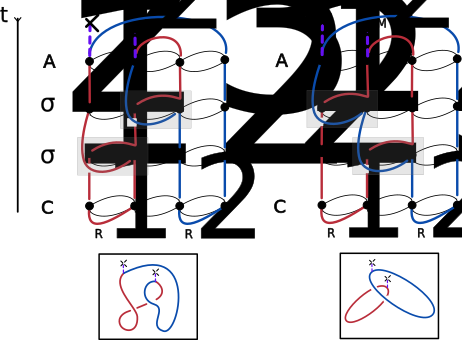
\includegraphics[width=\linewidth]{Figures/fluxBRAID.pdf}
    \caption{The two braiding protocols, differing only in order of exchange of two anyons. Protocol a) will have 4 fusion outcomes, while protocol b) can only produce vacuum.}
    \label{fig:flux_braid}
\end{figure}

Two pair of anyons are created from the vacuum, two interchanges are performed, and then the two pair are annihilated. 
In the first braiding, we annihilate the pairs that have a fixed fusion channel, given they are created from the vacuum they will fuse to the vacuum.
In the second braiding, we annihilate the pairs whose fusion channel is not fixed, hence all four outcomes are expected, the same result as in the fusion experiment.

The anyons we will braid are again pure fluxes $\Psi_m$, out of concreteness. The numerical results are shown in Figure \ref{}.

\todo{Figure Braiding Results: Resutls showing the charge measurement for the two braiding protocols.}

\jovan{ToCont}

\subsection{Interferometry}

In order to access full data of the S- and T-matrix, amplitude and phase of its elements, we must devise an interference protocol.

There will be a controlling bit $c$, whose states are entangled with different braiding protocol after a specific protocol:
\begin{equation}
    \ket{\psi}_c\ket{\text{G.S.}} \rightarrow \ket{0}_c \ket{\Psi_0} + \ket{1}_c \ket{\Psi_1},
\end{equation}
where $\Psi_i$ are the two wave functions of the matter degrees of freedom corresponding to two braiding operations.

If the charge content of the two states is the same they may only differ by a constant, hence we can write:
\begin{equation}
    \ket{0}_c \ket{\Psi_0} + \ket{1}_c \ket{\Psi_1} = (\ket{0}_c + C_{01}\ket{1}_c)\ket{\Psi_0},
\end{equation}
and by the means of tomography on the control bit $c$ we can extract the relative constant $C_{01}$.

For a suitable choice of two braiding protocols, this constant can equal some element of S- (and T-) matrix, see Figure \ref{fig:intef_example}.

\begin{figure}
    \centering
    \includegraphics[width = \linewidth]{Figures/intef_example.pdf}
    \caption{A possible interferometry scheme for measuring the S-matrix elements. The two possible braiding are appropriately entangled with the controlling bit $c$, which is achieved by controlled ribbon operators.}
    \label{fig:intef_example}
\end{figure}

This superposition is constructed by conditional braiding, conditioned on the state of the control bit. 
The conditional braiding is achieved by applying conditional ribbon operators.
For example, we can condition the existence of a ribbon by making any unitary gate involved in applying the ribbon operator conditioned on the state of the control bit.
Every, single qubit gate becomes a two qubit gate and every two qubit gate becomes a three qubit gate (unitarily similar to a Toffoli gate), hence, the number of entangling gates grows fast.

A smarter alternative way is to condition the anyon flavour of the ribbon, a ribbon label that is. One just needs to look at two ribbon operators and identify where they differ, and condition only those operations. The result is illustrated in Figure \ref{fig:flavCond}.


\begin{figure}
\begin{equation*}
\begin{split}
\Qcircuit @C=0.5em @R=0.7em @!R{
\lstick{c} & \ctrl{1} & \qw\\
\lstick{m} & \targ & \qw \\
\lstick{R} & \qw  & \qw \\
\lstick{R^{2}} & \targ  & \qw \\
\lstick{\text{aux}} &  \ctrl{-1} & \qw
}\qquad\qquad
\Qcircuit @C=0.5em @R=0.7em @!R{
\lstick{c} & \ctrl{2} & \qw\\
\lstick{m} & \qw & \qw \\
\lstick{R} & \ctrl{2}  & \qw \\
\lstick{R^{2}} & \qw  & \qw \\
\lstick{\text{aux}} &  \targ & \qw
}
\end{split}
\end{equation*}
\caption{The compiled ribbon operators, where the flavour of the ribbon is conditioned on the state of the control bit $c$. Left: controlled multiply circuit used when anyon moves along a leg $i$ encoded by the middle three bits. Right: controlled conjugation circuit used when anyon crosses along a leg $i$ encoded by the middle three bits. The flavours involved are pure flux $\Psi_m$ for $\ket{1}_c$ and $0 \oplus \tilde{0}$ for $\ket{0}_c$. Note: ribbons can also be associated with reducible representations of $D(G)$ as long as they are closed, if we require a well-defined topological charge of the end state.}
\label{fig:flavCond}
\end{figure}

In that example, the control bit is selecting between two ribbon flavours, the pure flux $\Psi_m$ and the one labelled by a reducible two-dimensional representation $0 \oplus \tilde{0}$. One can also look at the case where we condition the existence of the ribbon, by making every gate controlled by qubit $c$, as also selecting between two flavours, $\Psi_m$ and $0 \oplus 0$, the previous scheme simplifying the multiplication past of the circuit, Figure \ref{fig:flavCond} Left.

We will use both schemes in out phase-sensitive S-matrix experiment.

\subsubsection{S-matrix elements}

\begin{figure}
    \centering
    \includegraphics[width=\linewidth]{Figures/intefFlav.pdf}
    \caption{Caption}
    \label{fig:my_label}
\end{figure}
\begin{figure}
    \centering
    \includegraphics[width=\linewidth]{Figures/intefEx.pdf}
    \caption{Caption}
    \label{fig:my_label}
\end{figure}
\begin{figure}
    \centering
    \includegraphics[width=\linewidth]{Figures/phaseCheck.pdf}
    \caption{Caption}
    \label{fig:my_label}
\end{figure}

\subsubsection{T-matrix elements}

\subsection{Comment on Numerical Experiments}

In this section, we provided numerical evidence for the feasibility of our proposal, i.e. a set of noisy quantum circuit simulations that show that the nonabelian braiding signatures are observable.

The simulations were done via Google's 'cirq\_google' python package running on Google's cloud computing platform 'Google Colab'. This package executes the quantum trajectory simulation of the circuit using the Kraus operators obtained from the direct Pauli Transfer Matrix tomography on various single and two qubit gates on the Sycamore chip \cite{}.


\section{$S_3$ Gauge Group}
\section{Conclusions and Outlook}

\bibliographystyle{plain}
\bibliography{bibliography}


\end{document}
